\section{Step-by-step time evolution}

For a time-dependent Hamiltonian, an expansion in stationary eigenstates does not work in the same simple fashion. This is because the states $\psi_i$ are eigenvectors of the \textit{instantaneous} Hamiltonian. For different times , these vectors are not any more eigenvectors of the full Hamiltonian. 
That being said, with a step-by-step implementation we should get rid of the apparent degeneracy of the eigenvalues. 

\subsection{Euler scheme}
We now implement the Euler scheme for evaluating its applicability for the quantum problem. An interesting phenomena occur, where the function abruptly breaks down after a number of time steps. The approach to finding the number of steps before this breakdown is by looking at the normalization of the wave function. As this suddenly diverges, we can use this as a check in a while-loop for comparing step sizes in both temporal and spatial direction. 
\begin{figure}
	\centering
	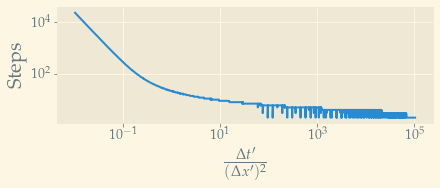
\includegraphics[width=\linewidth]{img/cfl.png}
	\caption{The number of steps taken before the Wave Function breaks down against the Courant-Friedrichs-Lewy (CFL)-number on a log-log scale.}
	\label{fig:cfl}
\end{figure}

In \cref{fig:cfl} the steps before the breakdown of the simulation for the Euler-Scheme is shown. This suggests that for the a successful simulation in this scheme, we need $\Delta t' \ll (\Delta x')^2$. At thee same time we also want $\Delta x' \ll 1$, so this would require a very heavy computation. A better approach is to use a different numerical scheme. 

 
\subsection{Crank-Nicolson}

The implementation of this scheme is done by computing the LU-decomposition of $\left(1+\frac{i}{2}\Delta t'\hat H\right)$ and solving a linear system $A\vb x= b$ for each time step. 
As previously mentioned, we should get rid of the degeneracy of states. With this in mind, the phase  $\sim \frac{1}{\lambda_2-\lambda_1}$ should diverge, and we have to propagate the system infinitely in time.  By preparing the same state as in \cref{eq:psi0}, we can use the Crank-Nicolson scheme to propagate the function and check this. 
\begin{figure}
	\centering
	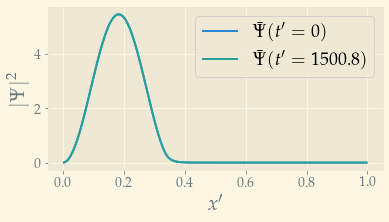
\includegraphics[width=\linewidth]{img/crank.png}
	\caption{Initial state and time-evolved state using the Crank-Nicolson scheme. }
	\label{fig:crank}
\end{figure}
As viewed in \cref{fig:crank}, there is now no tunneling, as opposed to the case when we project the states on a plane-wave basis, c.f. \cref{fig:tunneling}.

\subsection{Two level system}

\cref{fig:e1e2} shows the two lowest lying energy eigenvalues for $V(x, t)$ as introduced in  ref.\cite{assignment}. For $\nu_r = 0$, the energy difference is $\varepsilon_0 \simeq 5.6962$. 
\begin{figure}
	\centering
	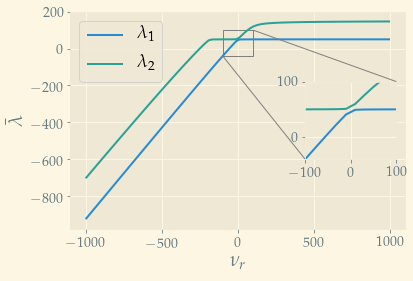
\includegraphics[width=\linewidth]{img/e1_e2.png}
	\caption{The two lowest eigenvalues plotted against the varying potential $\nu_r$. }
	\label{fig:e1e2}
\end{figure}

The expectation value 
\begin{equation} 
\tau = \mel{g_0}{\hat H}{e_0}
\end{equation}
can be computed as the previous inner products, applying first the action of $\hat H$ to $\ket{e_0}$ and then taking the inner product. $\tau$ is found to take a linear shape 
\begin{equation}
	\tau(\nu_r) \simeq -0.429\nu_r.
\end{equation}

